\documentclass[12pt,letterpaper]{article}
\usepackage[utf8]{inputenc}
\usepackage{amsmath}
\usepackage{amsfonts}
\usepackage{amssymb}
\usepackage{graphicx}
\usepackage{url}
\usepackage{wrapfig}
\usepackage[backend=bibtex,style=authoryear]{biblatex}
\addbibresource{bib/tm.bib}
%\usepackage{fullpage}
\usepackage[draft]{fixme}
\fxsetup{theme=color}
\author{}
\title{Nublu: A Vision for Data-centric Cloud Security}
\begin{document}
\maketitle
\section{Introduction}
\label{sec:intro}
Currently, the security of networked infrastructures tends to be managed statically. That is, security requirements are developed and implemented within the networking environment, and all of the information that traverses the network will have these hard-coded security policies applied to it. Thus, the security policies applied to all information is "one-size-fits-all", and can typically only be modified by network administrators. The result is that if there is a mismatch between mission requirements and network security, the network resources simply cannot be used to service the mission.

The ability to quickly, securely, and reliably share information across security domains is a capability that must be developed in order to ensure mission success in Department of Defence (DoD)cloud-based network-centric environments. We propose the continued development of an assured information-sharing framework for cloud-based systems that leverages our ongoing work in the areas of policy-based usage management and semantic interoperability. The development of this framework involves research related to the creation of a novel approach to information sharing that treats security as a commodity that can be dynamically provisioned within the cloud, along with other cloud resources.

\paragraph{Policy Tools.} First, we must develop the technologies that allow administrators to easily generate policies that leverage cloud computing-specific capabilities. That is, additional research is needed to develop a set of cloud computing-specific security policies that can be encoded into the extensible markup language (XML) policy format we currently use. This work will include extending our existing policy generator capabilities to address these cloud specific policies.

\paragraph{Dynamic Evaluation.} In addition, the usage management framework must be extended to include the ability to formally interpret and enforce cloud-specific policies. These capabilities must include the ability to dynamically monitor the policies associated with resources in use in order to immediately react to changes. We envision this research including the development of a satellite usage management capability that operates in each VM. This approach will also require the development of capabilities that allow the global usage management mechanism to communicate in an assured manner with the usage management mechanisms executing in the individual VMs, providing comprehensive usage control across a distributed cloud environments.

\paragraph{Enforcement.} Finally, policy enforcement mechanisms are needed at all levels of the cloud hierarchy to control how data and services are used. For example, if a data item is specified at a certain level of sensitivity, the usage management mechanisms must ensure that this item is not stored or routed through the cloud infrastructure in a way that would violate the policies associated with its sensitivity level. In order to accomplish this, our approach maintains clean separations between policy specification, interpretation and enforcement. This allows the framework to leverage security capabilities that are currently available or in development by other information security research groups.

\paragraph{Security Primitives and Control.} In general, a DoD cloud computing infrastructure may be highly heterogeneous and used by multiple parties that may be involved in multiple missions, leading to highly complex usage patterns and security requirements. Thus, our Phase II research will continue to investigate the use of control theory in order to ensure that multiple missions can be simultaneously satisfied within a given infrastructure. Our next steps in this area involve investigating VM performance control capabilities that enable monitoring of central processing unit utilization and the development of appropriate control algorithms that automatically add or remove VMs to meet performance requirements within a given security posture.

Additional security issues associated with cloud computing that will be considered as a part of this usage management/control-theoretic framework include joint tenancy of a not trusted user's VM on the same server hardware, data remnants in cloud storage repositories and VMs, and the trust associated with cloud provider?s administrators (who have complete access to user data and VMs). Some of these concerns could potentially be addressed with usage policies; however, further research is needed to explore how the proposed usage management framework, in conjunction with

\section{Operational Scenarios and Requirements}
\label{section:req-scen}
Nublu is intended to provide assured information sharing capabilities over private and public infrastructures.  To do this, we will provide a secure virtualized system protected by integrated policy-based usage management integrated with key encryption technologies.  Virtualization will span the entire system, from data repositories to communication networks to application servers to clients, when possible.

\subsection{Abstract Requirements}
\label{sec:requirements}
%\fxnote*{What other abstract requirements do we want to list?}{We currently have a group of abstract requirements the system must fulfil to be useful.  These address things like complete infrastructure virtualization to policy creation:}
This is an abstract list of requirements that describe how Nublu will support assured information sharing.  These individual requirements are very general and could be broken down into multiple, more granular requirements as needed.
\begin{itemize}
\item {\bf Flexible Infrastructure Provisioning} --- Infrastructure must be able to be provisioned without human intervention.

\item {\bf Dynamic Infrastructure Provisioning} --- Networks and systems must be able to be created and destroyed automatically based on need.

\item {\bf Data-driven Security Application} --- Security services must be applied to information based on characteristics of that information, associated policies, and environmental context.

\item {\bf Automated Security Services} --- Security services must be able to be applied without human intervention.

\item {\bf Automated Performance Tuning} --- System performance must be tunable by the system without human intervention.

\item {\bf Virtualized Infrastructure} --- Infrastructure must be completely virtualized in order to support dynamic allocation and provisioning.

\item {\bf Easy Policy Creation} --- The system needs tools that enable automated policy creation whenever possible based on either none or some small amount of entered information.
\end{itemize}

\subsection{Selected Scenarios}
\label{sec:scenarios}
%\fxnote*{These need to be elaborated, but how much?}{We have specific scenarios that embody information sharing that we can use to highlight the kind of functionality the system needs to produce in order to provide assured cloud-based information sharing.  These scenarios have distributed communication requirements, use encryption, have multiple parties of various trust levels and need to know, and use both human and machine agents.}
Nublu will enable multiple scenarios, flexibly securing information as it is collected and disseminated.  These range from streaming data collection, do limited data consumption, to block transfer supported by storage systems in a datacenter.s

\paragraph{Streaming Data From Drone.} This is a data ingestion scenario.  Data from some kind of drone, manned or unmanned, is pulled into a cloud-centric distribution system for storage and processing.

\paragraph{Streaming Data Consumption by Coalition Partner.} In this scenario, a coalition partner is streaming video from a data source to some type of client. The video itself is not classified, but it is sensitive, and is accompanied by specific usage and routing policies.

\paragraph{Block Data Transfer within Datacenter.} Datacenters in cloud environments usually host block storage for cloud clients on systems that are distinct from the computational systems themselves.  Here, filesystem blocks are transferred from a block store to a client.  The blocks themselves are categorized as sensitive, and have associated usage and management policies.

\paragraph{Automated Information Consumption by Remote System Agent.} Here, a system agent on a remote system acquires data from a variety of cloud services for analysis.  The agent itself is authenticated and authorized to access information, and the secondary data resulting from the analysis is saved and protected by usage policies that provide provenance information pointing to the original data used.

\paragraph{U.S. Operator Information Creation.} In this scenario, a remote operator in the field creates some kind of data record.  This record can be either an audio, video, or document-centric record.  The information is saved with a default policy based on information gathered automatically from the creation location and user authentication information as well as a small amount of information entered by the user.

\section{Solution Overview}
\label{sec:overview}
We will use a simple model to begin development.  We have three distinct layers --- {\sl application}, {\sl logical}, and {\sl physical} layers. This application layer consists of {\sl data repositories}, {\sl communication networks}, {\sl application servers}, and {\sl clients}.  The logical layer contains {\sl images} and {\sl instances} running in {\sl containers}, while the physical layer contains all physical hardware and software required to enable the logical layer.

These can be combined into common {\sl patterns}, including:
\begin{itemize}
\item Intra-datacenter
\item Inter-datacenter
\item Datacenter to cache
\item Datacenter to application server
\item Datacenter to client
\item Cache to application server
\item Cache to client
\end{itemize}
All these communication patterns have distinct {\sl trust profiles}.

\subsection{Major Features}
\label{sec:features}
%\fxnote*{Should this have a conops perspective? What's the appropriate depth?}{The major system features differentiating this approach from other information sharing approaches is the scale of the system, the system's flexibility, and integrated content usage management.}
To flexibly provision security based on data and context rather than system, Nublu must be flexible, scale across sensitivity levels as well as system demand, and provide easy to use usage management primitives.

\begin{wrapfigure}[25]{r}{.5\textwidth}
\begin{center}
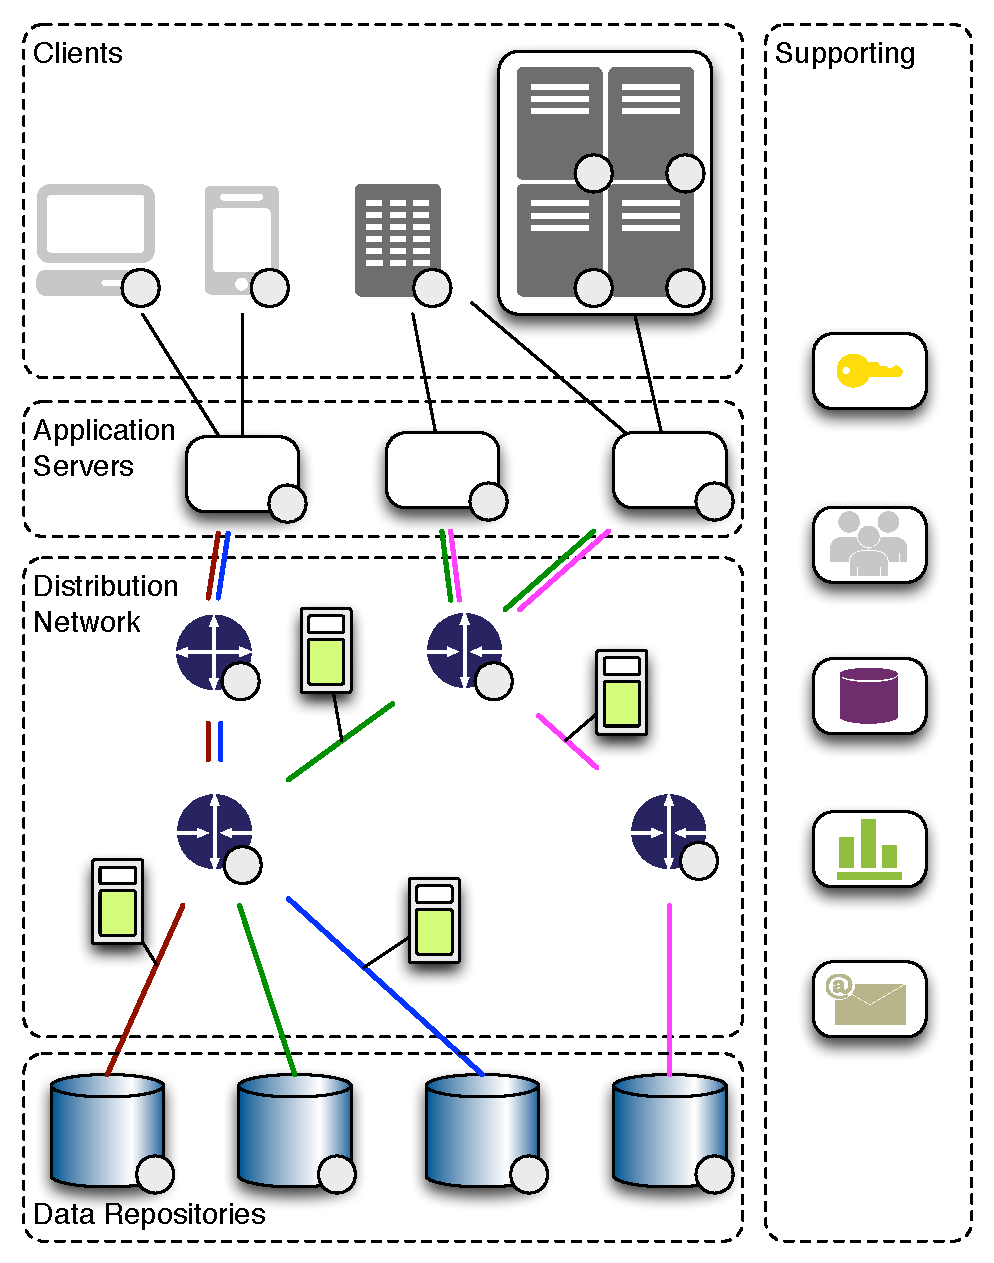
\includegraphics[width=.47\textwidth]{./images/network.pdf}
\end{center}
\caption{A notional view of the Nublu system, showing various required and provided services in an end-to-end perspective.}
\label{fig:network}
\end{wrapfigure}

\paragraph{System Scale.} Unlike other information environments like SIPRNet or JWICS, this system will prototype the ability to store information from a single system at a variety of classification and sensitivity levels via integrated encryption.  Furthermore, this system will operate as a cloud computing environment with the scalability that implies~\footfullcite{nist-sp-800-145}.

\paragraph{System Flexibility.} The system will allow policies to be evaluated within a dynamic context.  For example, under cases of duress, the system may elect to transmit sensitive information to users that would generally not be allowed access to that information.  This information would be shared in such a way that it could be retracted at a later date, and the system would create traceable records outlining which users received the information.  In addition to this information management flexibility, the system will also support the kind of operational flexibility expected of cloud systems~\footfullcite{nist-sp-800-145}.

\paragraph{Content Usage Management.} Nublu will enable management of information content throughout the system and information life-cycle.

\subsubsection{Within the Datacenter}
Modern computational infrastructures supporting virtualization have changed radically from the types of server-class systems used in the past.  Systems from a decade ago would be more integrated and have physical capabilities built directly into the physical system that virtualized systems do not have today. For example, a server system without a generous amount of secondary (i.e. disk) storage would be unheard of ten years ago.  Today, this absence of on-board non-volatile is common in cloud systems, and is expected when provisioning systems from commercial providers.  In fact, this has given system designers more options when designing virtualized hosts, allowing them to select the performance of virtual secondary storage from a range of performance and price points.

To understand how to partition images within a cloud datacenter, we must have some idea of how a datacenter would typically be assembled.  These systems are partitioned into servers of various capabilties, providing a variety of services, including storage, processing, security, and network management.  These servers are stored within a rack, with a switch (i.e. a top-of-rack switch) handling local traffic within the rack.  Server densities, system power, and switch capabilities within and between racks may vary, but this construction pattern is typical of a single rack.

These racks can then be organized into a cluster of some kind.  These clusters may be contained within shipping containers, or similar enclosures.  These enclosures are then assembled into a datacenter, linked to other datacenters via ISPs.

Within a given datacenter however, different types of servers will be provisioned for different types of services.  These servers are built expressly for their intended purpose --- they may be constructed of general purpose computing components, but the profile the components are in is very specific to a given task.  Some servers are designed for fast processing, with multiple cores, fast cache, and high performance drives.  Others may be dedicated to storage, with massive arrays of drives made available to other systems over the network.  Still others may be dedicated to queueing, and others for long-term inexpensive storage.

These systems work together to provide virtual machines and supporting services.  Nublu will use these kind of components to enable data-centric, context-sensitive security.  Various servers and services will be able to be re-provisioned in a variety of configurations to support computing needs at a wide range of sensitivity levels.  The network fabric itself, staring from the top-of-rack switches, will be able to isolate communications by sensitivity, need-to-know, and support responsibility-to-provide.  Storage systems will isolate information appropriately and be able to extend those protections through the network to virtual machines spun up to support dynamic, pop-up networks at various security levels.

\subsubsection{Between Datacenters}

\subsubsection{Client Perspectives}

\printbibliography

\end{document}